% =====================================================================
% TEMPLATE SWITCH: leave \naturetrue commented for LoG; uncomment it for
% Springer Nature / Nature Portfolio (sn-jnl class, sn-nature reference style).
% Everything below branches on \ifnature; nothing else needs editing.
% =====================================================================
\newif\ifnature
\newif\ifnatureprint
% \naturetrue
% \natureprinttrue	% with \naturetrue: preview at Nature's printed page width
						% (two 89 mm columns, 183 mm text block; figures span both columns)

% Both classes load xcolor; pass extra options here, before the class, to avoid an option clash.
\PassOptionsToPackage{table}{xcolor}        % \rowcolors / \rowcolor in tables

\ifnature
  % --- Springer Nature (template v3.1, Dec 2024) ---------------------------
  % sn-jnl already loads hyperref, geometry and natbib[numbers,sort&compress],
  % and sets \bibliographystyle{sn-nature}. Do NOT load natbib or hyperref yourself.
  % The submission template is a generic single column with a 31 pc (131 mm) text width,
  % not Nature's printed layout, so figures drawn at 183 mm are shown at ~72% size.
  \ifnatureprint
    \documentclass[pdflatex,sn-nature,iicol]{sn-jnl}
    \geometry{text={183mm,247mm},columnsep=5mm,bindingoffset=0mm,hcentering}
    \setlength\columnhsize{89mm}
  \else
    \documentclass[pdflatex,sn-nature]{sn-jnl}
    % \documentclass[pdflatex,sn-nature,lineno]{sn-jnl}	% with line numbers
    % \documentclass[pdflatex,sn-nature,referee]{sn-jnl}	% double-spaced referee copy
  \fi
  \usepackage{xcolor}
  \usepackage{amsmath}
  \hypersetup{bookmarksdepth=2}
\else
  % --- LoG 2025 --------------------------------------------------------------
  \documentclass{article}
  \usepackage{log_2025}						% for camera-ready version
  % \usepackage[review]{log_2025}			% for anonymous submission to proceedings track
  % \usepackage[review,eabstract]{log_2025}	% for anonymous submission to extended abstract track
  % \usepackage[preprint]{log_2025}			% for preprint version
  % \usepackage[eabstract]{log_2025}		% for accepted extended abstract papers
  % Citation colour: the style file sets citecolor=NavyBlue (near-black); override it here
  % (any xcolor svgnames colour, e.g. RoyalBlue, MediumBlue, Teal). Comment out for the default.
  \AtBeginDocument{\hypersetup{citecolor=RoyalBlue}}
  % First-page footer ("Proceedings of the ... Learning on Graphs Conference" / "Submitted to ...").
  % This line removes it; comment it out to restore the footer.
  \makeatletter\renewcommand{\@notice}{}\makeatother
  % NB: the style file already loads amsmath, microtype, xcolor, caption, geometry, url and
  % hyperref (at end of preamble). Do NOT \usepackage{hyperref} yourself.
  \usepackage{subcaption}					% (a)/(b) subfigures
  \usepackage[numbers,compress,sort]{natbib}	% for numerical citations
  % \usepackage[sort,round]{natbib}			% for textual citations
\fi

\usepackage{etoolbox}						% \AtEndPreamble (used for cleveref below)
\usepackage{booktabs}						% professional-quality tables
\usepackage{multirow}						% tabular cells spanning multiple rows
\usepackage{tabularx}						% fixed-width tables with X columns
\usepackage{amssymb}						% blackboard math symbols (superset of amsfonts)
\usepackage{bm}								% bold math
\usepackage{graphicx}						% figures
\graphicspath{{figures/}}					% figures are PDFs converted from the repo's SVGs
\usepackage{siunitx}						% \SI{3}{\second}; S table columns
\usepackage{soul}							% \hl highlighting for annotations
% \usepackage{algorithm}					% algorithm floats
% \usepackage{algpseudocode}				% pseudocode inside them
% \usepackage{tikz}							% schematics drawn in TikZ

% cleveref must load after hyperref (LoG loads it at end of preamble; sn-jnl in the class)
\AtEndPreamble{\usepackage[capitalise,nameinlink]{cleveref}}	% \cref{fig:x} -> "Figure 1"

% Back-matter headings: \bmhead in sn-jnl, unnumbered sections in LoG.
\ifnature
  \newcommand{\backhead}[1]{\bmhead{#1}}
\else
  \newcommand{\backhead}[1]{\section*{#1}}
\fi

% --- front matter (shared text) -------------------------------------------
% Title in Initial Caps; the optional argument is the running head.
\title[Dependence profiles]{Reading the Character of Dependence in Multivariate Time Series}

% Single paragraph, ideally 4--6 sentences (Nature Portfolio: check the journal's word limit, usually ~150--200 words, no citations).
\newcommand{\abstracttext}{%
A strong association between two signals can reflect shared fluctuations, delayed responses or dependence confined to particular amplitudes. Across a recording, these possibilities can be distinguished when statistics sensitive to different properties assign strength to different channel pairs. We represent each recording by the correlations between its edge profiles, one profile per statistic. Controlled changes in observation form and timing yield distinct signatures, and the representation separates nine simulated classes across recording sizes. In noisy oscillators, its leading component tracks the onset of cross-frequency locking even as recording quality dominates the leading component of mean edge strengths. In four macaques, Gaussian and nearest-neighbour estimates of mutual information agree less closely during anaesthesia than expected from the spectra of the same windows. Ketamine and propofol produce this change despite opposite shifts in mean excess information. A prespecified window selection during mouse isoflurane induction shows the same direction, as does propofol electrocorticography in six of seven patients. Together, these examples give recording-level descriptors an interpretation in terms of which properties of dependence distinguish one set of edges from another.%
}

\ifnature
  \author*[1]{\fnm{Will} \sur{Edibam}}\email{will.edibam@sydney.edu.au}
  \author[1]{\fnm{Ben D.} \sur{Fulcher}}
  \affil*[1]{\orgdiv{School of Physics}, \orgname{The University of Sydney}, \orgaddress{\city{Sydney}, \state{NSW}, \country{Australia}}}
  \abstract{\abstracttext}
  \keywords{multivariate time series, statistics of pairwise interactions, representation learning, dependence}
\else
  % Abbreviated author list in [ ] is used in the first-page footnote. Authors are hidden under [review].
  \author[W. Edibam and B. D. Fulcher]{%
  Will Edibam \and Ben D. Fulcher \\
  The University of Sydney \\
  \email{will.edibam@sydney.edu.au}
  }
\fi

\begin{document}

\maketitle
\ifnature\else
  \suppressfloats[t] % stop floats landing above the title on page 1
  \begin{abstract}
  \abstracttext
  \end{abstract}
\fi

\section{Introduction}

Consider a cortical recording in which neighbouring electrodes fluctuate together. A change in their correlation after anaesthesia tells us that the strength of their linear association has changed. It leaves open a question about the recording as a whole. Are the electrode pairs that share the most information still the ones whose signals are most closely correlated? The distinction matters even when every electrode can be matched between recordings. A drug could strengthen dependence on some pairs and weaken it on others while preserving the correspondence between the two measures. It could also change that correspondence, so that knowing which pairs are strongly correlated becomes a poorer guide to where information is shared.

Every measure of coupling makes a choice about what counts as an interaction. A covariance gives weight to simultaneous deviations from the mean. A lagged covariance asks whether a deviation in one signal precedes a deviation in another. Mutual information gives weight to any departure of the joint distribution from independence. Each supplies a set of edge strengths. The information gained by comparing them resides in the identity of the edges. Two measures can have identical distributions of strengths in two recordings and still disagree about the edges to which those strengths belong.

Comparisons of this kind already inform the study of dependence. Contrasts between linear and nonlinear redundancy test Gaussian descriptions of time series \cite{palus1995testing,hlinka2011functional}. Comparisons of phase and amplitude coupling reveal which spatial patterns recur across distinct physiological measures \cite{mostame2020phase,siems2020dissociated}. At catalogue scale, Cliff et al.\ compared the edge profiles of pairwise statistics across diverse systems, and Liu et al.\ compared functional connectivity measures across individuals \cite{cliff2023unifying,liu2025benchmarking}. Here we retain a signed profile correlation for each pair of statistics \emph{in each recording}. We ask which of these correspondences persists between recordings and which changes with state. A change can then be sought in the joint behaviour of many statistics, and a selected coordinate can be read against the particular difference between its two estimators.

We develop this argument at four levels. We first change the observation map or the timing of a shared signal and ask which statistic pairs respond. We next ask whether a common representation separates simulated dynamical families across channel counts and record lengths. In systems with a known order parameter, we test what a label-free coordinate tracks and when simple strength summaries recover the same transition. Finally, in cortical recordings, we examine a pair of estimators of the same quantity. Their agreement has a natural reference under Gaussian dependence, which makes the change during anaesthesia interpretable even though the underlying neural coupling function is unknown.

\begin{figure}[htbp]
\centering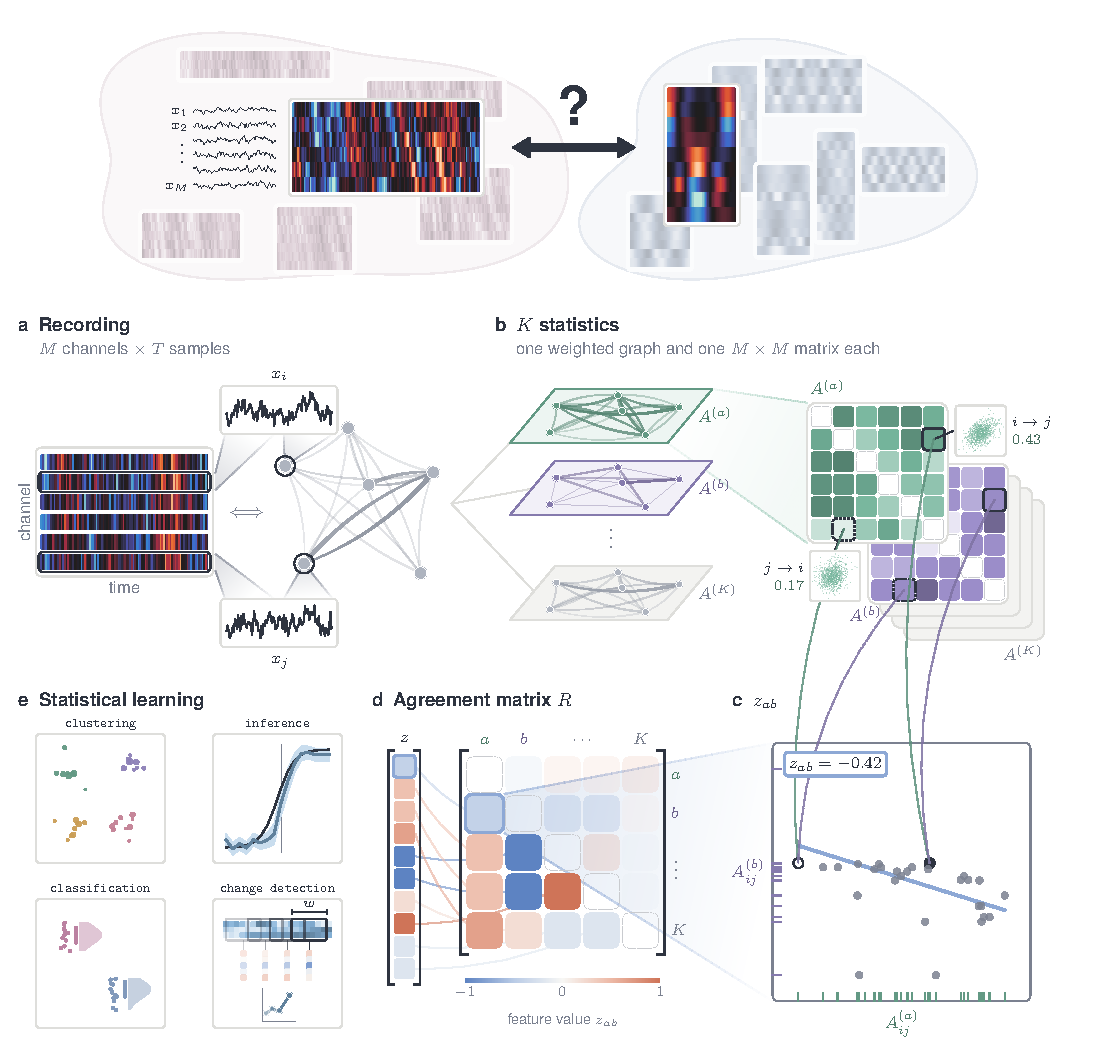
\includegraphics[width=\linewidth]{method-schematic-helvetica}	% 2026-11-18 schematic (commit cc7970a9), Helvetica rendition
% \centering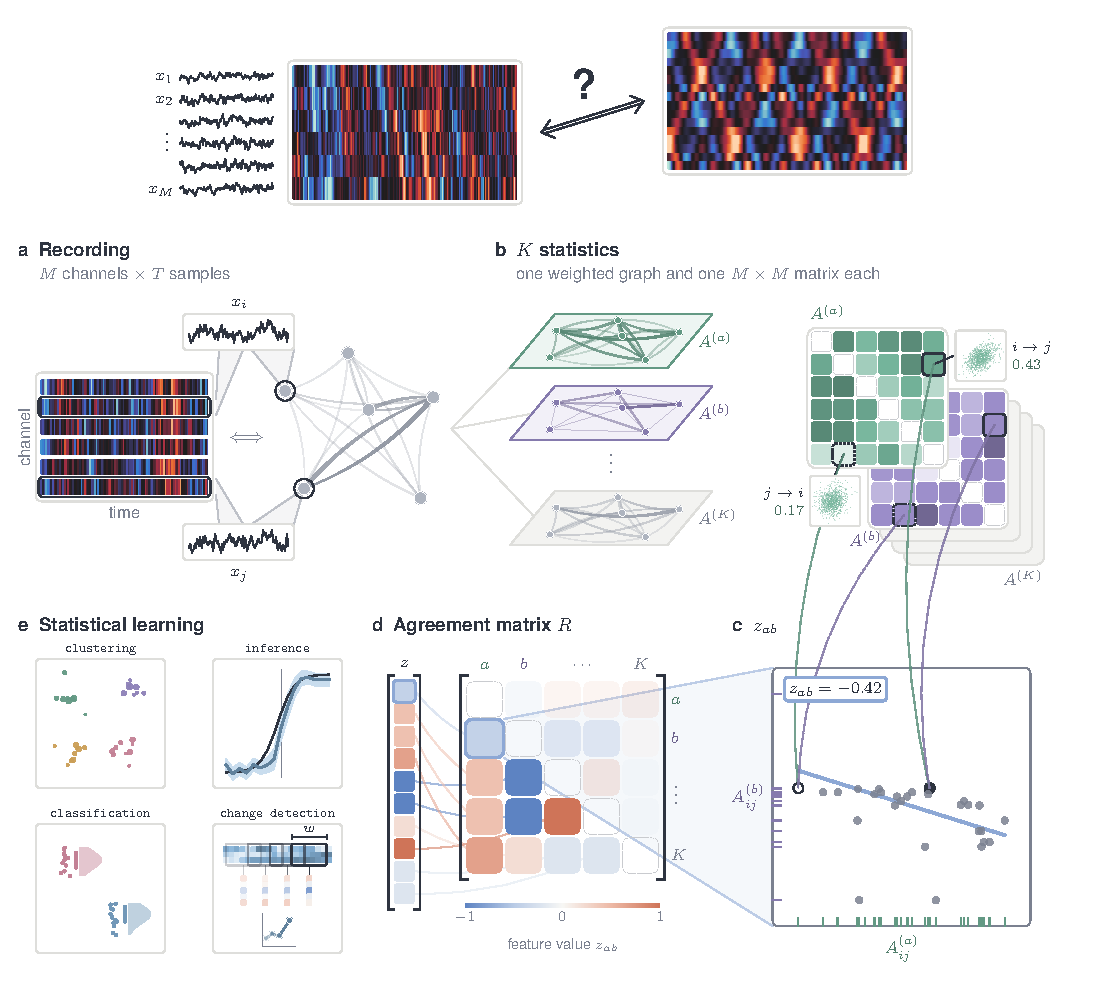
\includegraphics[width=\linewidth]{method-schematic}		% previous schematic (2026-10-30), outdated
\caption{\textbf{From channels to a recording descriptor.} Each statistic assigns a value to every ordered pair of distinct channels. The values for one statistic form an edge profile. Aligning two profiles by channel pair gives one point per edge in their scatterplot and one correlation per recording. Statistic identities supply the common coordinates when recordings differ in sensor identity or count.}
\label{fig:method}
\end{figure}

\ifnature\else\section{Methods}
\label{sec:methods}

\paragraph{Edge profiles and their agreement.}
For a recording $X\in\mathbb{R}^{T\times M}$ and statistic $a$, let $v_a$ list its values $A^{(a)}_{ij}$ over all $i\ne j$ in a common order. Directed statistics retain both orientations. Duplicating the two orientations of an undirected pair leaves its correlation with another undirected profile unchanged. We define
\begin{equation}
z_{ab}=\frac{\langle v_a-\bar v_a,\ v_b-\bar v_b\rangle}{\|v_a-\bar v_a\|\,\|v_b-\bar v_b\|}.
\label{eq:z}
\end{equation}
The $K(K-1)/2$ coordinates of a $K$-statistic catalogue describe how estimates covary across edges. Pearson correlation preserves the sign and linearity of this correspondence. A common permutation of edge entries, including a channel relabelling, leaves the descriptor unchanged. A positive affine transformation of either profile also leaves it unchanged. Changing physical coupling can still reshape a profile and move $z$. A constant profile has undefined coordinates; nearly constant or unreliable profiles can give unstable ones. In the catalogue analysis we exclude invalid profiles for the recording and handle missing coordinates at the analysis stage. The edge count sets the dimension over which a correlation is measured and supplies no independent experimental replicates.

\paragraph{Controlled perturbations.}
The form experiment used 12 channels in blocks of four and $T=2000$. A common standardised AR(1) signal $u$ (coefficient $0.8$) was mixed with independent Gaussian channel noise, $w_i=(u+s_i\epsilon_i)/\sqrt{1+s_i^2}$, with the same four log-spaced noise levels $0.2$--$1.0$ per block. The first block observed $w_i$, the second either $w_i$ or $\sinh(2w_i)$, and the third either $w_i$ or $w_i^2$. After channel standardisation we computed empirical covariance (Pearson correlation), Spearman correlation and four-neighbour Kraskov MI \cite{kraskov2004}. The timing experiment used 15 channels in blocks of five and $T=1000$. Channels sampled a common smooth Ornstein--Uhlenbeck signal at $t-d_i(t)$ with additive noise. One block was aligned, one aligned or delayed by one to five samples, and one aligned or warped with $d_i(t)=A_i\sin(2\pi t/250)$ for $A_i=2,4,6,8,10$ samples. Every block used the same noise schedule ($0.1$--$0.4$). We compared normalised Euclidean distance, the minimum Euclidean distance over constant shifts (up to 250 samples), and normalised dynamic time warping. Each design used 20 independent seeds with paired draws across the four configurations.

\paragraph{Generative classification.}
The nine classes comprised independent Gaussian or Cauchy noise, two ring vector autoregressions, fast or slow repulsively coupled Kuramoto oscillators, two quadratic coupled map lattices, and a periodic one-dimensional wave equation. Each had ten realisations for every $(M,T)\in\{8,16,32\}\times\{500,1000,2000\}$. For the two autoregressions, self and per-neighbour coefficients were $(0.7,0.1)$ or $(0.2,0.35)$. The lattice map parameter and coupling were $(1.7522,0.00115)$ for intermittency and $(2,0.3)$ for developed turbulence. From the 283-statistic proof catalogue we reconstructed ordered edge-profile coordinates, kept those finite in at least 95\% of recordings, median-imputed missing values and removed coordinates of variance at most $10^{-8}$. The centred matrix yielded 50 principal components. The display used openTSNE 1.0.4, perplexity 30, five degrees of freedom and PCA initialisation (seed 260924). In a descriptive size-cell audit, the nearest-neighbour classifier excluded the target cell, but the unsupervised preprocessing and PCA saw all displayed recordings. For each within-family comparison we chose an interpretable coordinate with oriented training AUC at least $0.995$ in every size cell on instances 0--5. Instances 6--9 were used only for its displayed distributions and AUC.

\paragraph{Physical order.}
In the locking model, populations A and B of eight oscillators each interact through $2{:}1$ resonant coupling \cite{komarov2015}; a third eight-oscillator population has internal coupling only. We observed $\sin(\phi_i)$ for $1000$ samples and varied the A--B coupling over $0,0.01,\ldots,0.20$. The physical target was $Q=|\langle\exp[i(\Psi_B-2\Psi_A)]\rangle|$ from collective phases over a disjoint future interval. In the variable-noise arm, independent white measurement noise had one recording-specific standard deviation drawn uniformly from $0.3$--$0.9$ signal standard deviations. At each coupling eight independent seeds fitted the readouts and eight evaluated them. PCA used centred coordinates for $z$, and standardised edge means for the comparator from the same 289-statistic historical catalogue. The targets supplied an orientation for display. The Stuart--Landau comparison used 32 oscillators, coupling $0.8$, and a fine population-parameter sweep $0.680$--$0.770$ against mean phase coherence. The lattice comparison used 32 dispersed sites on a $256\times256$ lattice against a full-lattice period-two order parameter. Both used independently generated confirmation records. In the electronic oscillator data of Vera-\'{A}vila et al.\ \cite{vera2026}, carrier-frequency range indexed locking; the Erd\H{o}s--R\'enyi sweep supplied the fit and the small-world sweep a transfer comparison.

\paragraph{Gaussian reference and nonparametric MI.}
In each empirical MI window we normal-scored channel $i$ by $\Phi^{-1}[(\operatorname{rank}(x_i)-1/2)/T]$. For edge $e$ with normal-score correlation $r_e$, let $G_e=-\frac12\log(1-r_e^2)$ in nats. For continuous population variables with standard normal marginals and finite MI, $I_e-G_e=D_{\rm KL}(P_e\Vert\mathcal{N}(0,\Sigma_e))\geq0$, where $\Sigma_e$ is their nonsingular covariance matrix \cite{ince2017}. To see this, the Gaussian reference has the same marginal entropies and its log density is quadratic, with identical expectation under both distributions. The joint entropy difference is therefore precisely the KL divergence. The identity applies to population MI. Our flexible estimate $K_e$ used the same observations, four nearest neighbours and a pair-specific temporal exclusion radius from the autocorrelation functions (twice their inner product, integer-truncated and capped at $T/10$). Sampling error and estimator bias can give $K_e<G_e$.

\paragraph{Empirical windows, controls and unit of analysis.}
The NeuroTycho analysis used electrocorticography from four macaques \cite{yanagawa2013}. Signals were notch-filtered at mains frequency, band-limited to $0.5$--$40$ Hz, downsampled to 100 Hz and referenced to the mean of the retained channels. Nonoverlapping 10-s windows passed the atlas artefact screens. We compared eyes-closed wake with drug or sleep within each date, with eyes-open wake and recovery where available. The primary MI analysis used 32 dispersed contacts (496 undirected edges) and one multivariate iterative amplitude-adjusted Fourier-transform (IAAFT) surrogate per window. The final Fourier step retains each channel's spectrum and the between-channel phase differences at each frequency, hence the cross-spectra, while matching the normal-scored marginals approximately \cite{prichard1994generating,schreiber2000surrogate}. It randomises aspects of within-window timing that those constraints leave free. We averaged $R=z(G,K)_{\rm observed}-z(G,K)_{\rm surrogate}$ over windows within each date and state, then compared states within date and summarised dates within animal. An all-channel follow-up used three joint draws. Matched surrogates calibrate finite-window performance; one draw per window gives no tail probability for an individual edge or window.

In mouse isoflurane EEG (DANDI 000458), the induction follow-up required at least three stimulus-free windows with burst index (MAD/SD) at or above the awake fifth percentile and delta fraction at or above the awake 95th percentile for that animal. Nine of 17 mice qualified. The reference comprised its awake windows; three joint surrogates per window supplied the null and the interval resampled mice. The human comparison used pre-infusion and sub-anaesthetic infusion stereo-EEG from seven patients (DANDI 001347). Cross-species tests use participants as replicates and address the specified exposure and measurement conditions.

\paragraph{Reproducible lead--lag structure.}
At lag $\tau$ we computed the ordered matrix $C_{ij}=\operatorname{corr}(x_i(t),x_j(t+\tau))$. For each unordered edge set $S=(C_{ij}+C_{ji})/2$ and $A=(C_{ij}-C_{ji})/2$, orienting edges consistently across windows. Reversal of time exchanges $C$ and $C^\top$. With $S_c$ centred over unordered edges and $U=\|A\|^2$, $V=\|S_c\|^2$, the antisymmetric fraction $U/(U+V)$ equals $(1-z(C,C^\top))/2$ exactly on ordered edges. To measure the repeatable part, we replaced each mean square by the average dot product of the corresponding edge maps from distinct windows in the same date and state, divided by the number of edges. This removes the within-window noise square; correlated fluctuations across windows may still contribute. We report asymmetric energy and its fraction of repeatable total energy separately. The primary lag was 20 ms, with 10 and 40 ms as sensitivities. We used 32 dispersed channels and repeated the measurement on 32 disjoint index-neighbour bipolar differences. Post hoc checks used all retained channels and a Fourier reconstruction fixing each dispersed channel's amplitude spectrum to its date-specific root-mean-square awake spectrum while retaining its window-specific phases.

\paragraph{Data and implementations.}
Macaque data are from NeuroTycho. Mouse and human data are available from DANDI (000458 and 001347). The hardware sweeps are Zenodo records 17451096 and 17451530. The study repository contains the form and delay generators, the nine-class proof configuration, the locking and companion benchmark protocols, and the recording-level analysis scripts. The empirical MI calculation uses an explicit nearest-neighbour implementation with temporal exclusion. The lag calculation operates directly on the retained time series. Neither requires estimating the remainder of the SPI catalogue.
\fi

\section{Results}

\subsection{Two contrasts distinguish observation form and timing}

A monotone distortion provides a case in which the outcome can be predicted edge by edge. Each channel observed a noisy version of the same Gaussian signal. Applying $g(w)=\sinh(2w)$ to one block preserves the ranks of its samples and the information shared with every other channel. It can nevertheless change Pearson correlation by different amounts on different edges. Across 20 realisations, mean $z(r,\rho)$ fell from $1.000$ to $0.500$, while $z(\rho,\mathrm{MI})$ moved only from $0.942$ to $0.939$ (\cref{fig:form}). The recording changed under observation through a different marginal scale, although its copula was preserved.

Folding one block instead, $g(w)=w^2$, produced a different signature. For a folded and an untransformed channel, the sign of the latent fluctuation cancels out of both Pearson and rank correlation by symmetry. Its magnitude still carries information. Mean $z(r,\rho)$ remained $0.995$, while $z(\rho,\mathrm{MI})$ fell to $0.622$. With both transformations present the coordinates were $0.874$ and $0.618$. These two readings are calibrated to the specified perturbations. In particular, the first example shows why raw Pearson--rank disagreement alone is an ambiguous indicator of a change in the dependence copula.

\begin{figure}[htbp]
\centering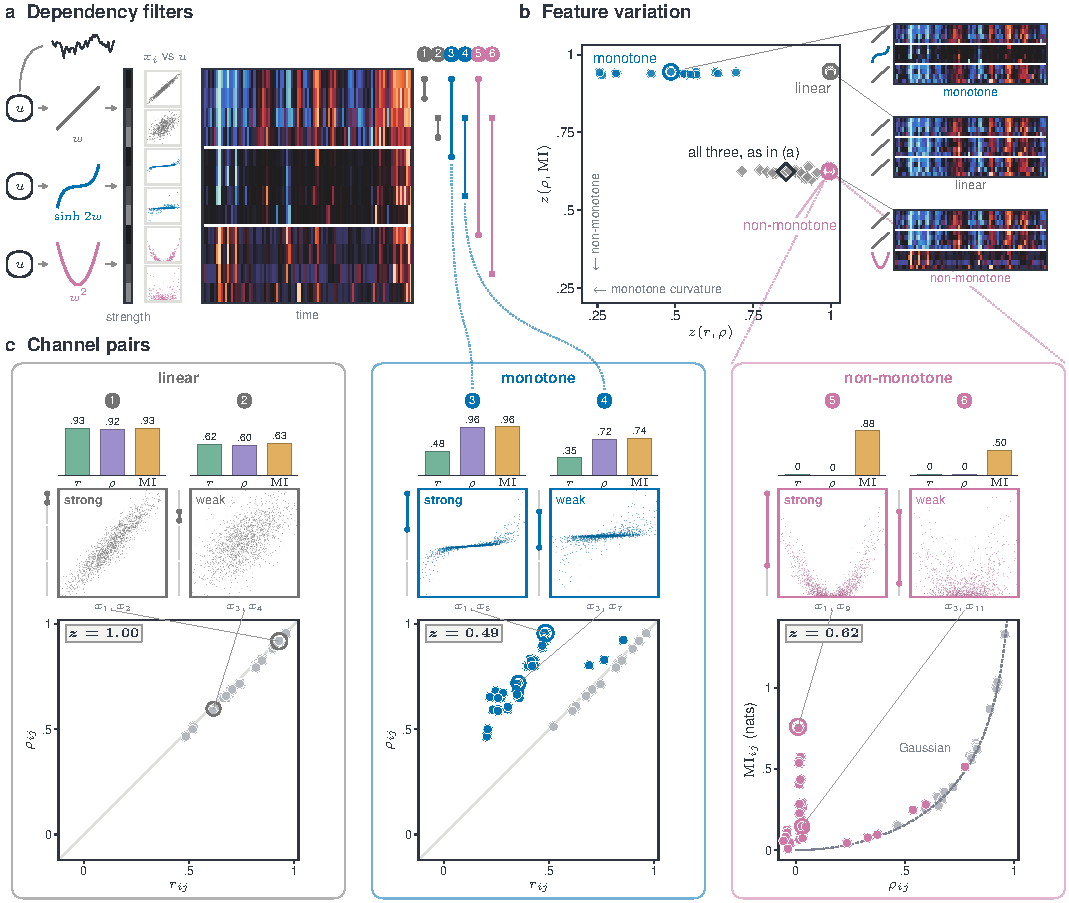
\includegraphics[width=\linewidth]{case-form-ladder}
\caption{\textbf{Changing how a common signal is observed.} Blocks apply linear, monotone or folded maps to signals with the same latent noise schedule (a). Each recording has two coordinates (b). Edge-level views (c) show how the monotone block moves points away from Pearson--rank agreement, and how folded edges can retain information at small rank correlation.}
\label{fig:form}
\end{figure}

Timing affords a corresponding experiment without changing the observation map. One distance compared signals sample by sample (ED), a second allowed a constant shift (xED), and a third allowed the alignment to vary in time (DTW). All three closely agreed when channels were aligned. Giving one block fixed delays reduced $z(\mathrm{ED},\mathrm{xED})$ from $1.000$ to $0.264$, with $z(\mathrm{xED},\mathrm{DTW})$ at $0.990$. Smoothly varying the delay produced the complementary pattern, $0.999$ and $0.426$. When both kinds of delay were present, the coordinates were $0.623$ and $0.420$ (\cref{fig:timing}). Agreement shifted at the comparison whose alignment rule mattered for the affected pairs. This identifies which tolerance changed the organisation of the distance estimates, without estimating a conduction delay from their correlation.

\begin{figure}[htbp]
\centering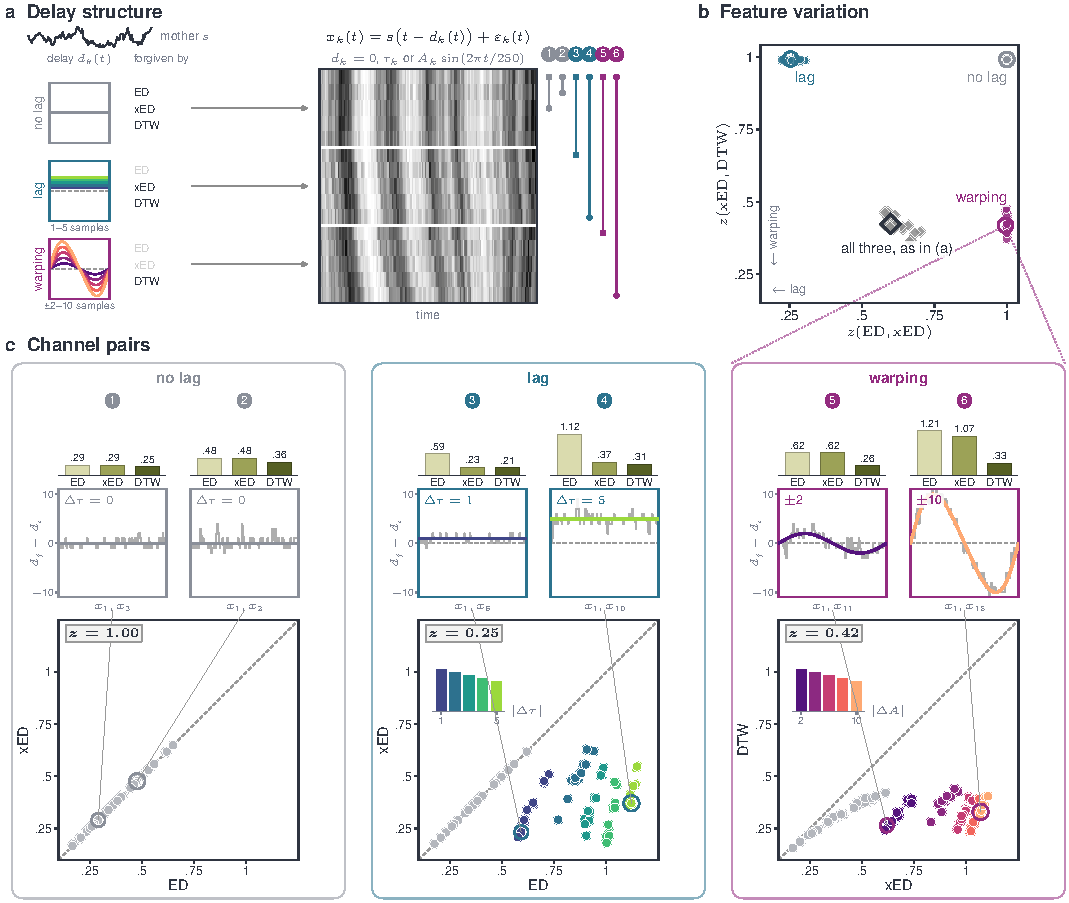
\includegraphics[width=\linewidth]{case-drift-blocks}
\caption{\textbf{Constant and varying delays separate along different coordinates.} Signals share one smooth trajectory. In a lagged block, a fixed shift aligns it across channels. In a warped block the appropriate shift varies throughout the record (a). Coordinates for 20 realisations per condition (b) are built from the distances of individual channel pairs (c).}
\label{fig:timing}
\end{figure}

\subsection{A common set of coordinates separates nine generative classes}

We applied the representation to 810 recordings spanning independent noises, vector autoregressions, coupled oscillators, coupled map lattices and a wave equation. Within several families even the coupling graph is identical across variants. The two autoregressions, for instance, have the same ring, spectral radius and total weight. They differ in how much of that weight is assigned to a channel's own past. Across three channel counts and three record lengths, recordings grouped by generator in a common embedding (\cref{fig:proof}). In the 50-dimensional principal-component space underlying the display, five nearest neighbours from other size cells classified 808 of 810 recordings correctly. All cells contributed to the unsupervised projection.

Individual coordinates help explain the separation. In the ring autoregressions, lagged MI credits information shared by the source's past and target's present. Transfer entropy asks how much the source adds once the target's own past is known. Moving weight between self-memory and neighbours changes the correspondence between these profiles. In the lattice maps, even the choice of one versus two time steps separates intermittency from developed turbulence. For each of four within-family contrasts, a coordinate selected on six instances per cell perfectly ordered the remaining four per cell (36 recordings per variant, AUC $1.00$). Selection used class labels. The result establishes separation for the specified generators; in the independent-noise example, it is variation in sample correlations under heavy tails that supplies the signal.

\begin{figure}[htbp]
\centering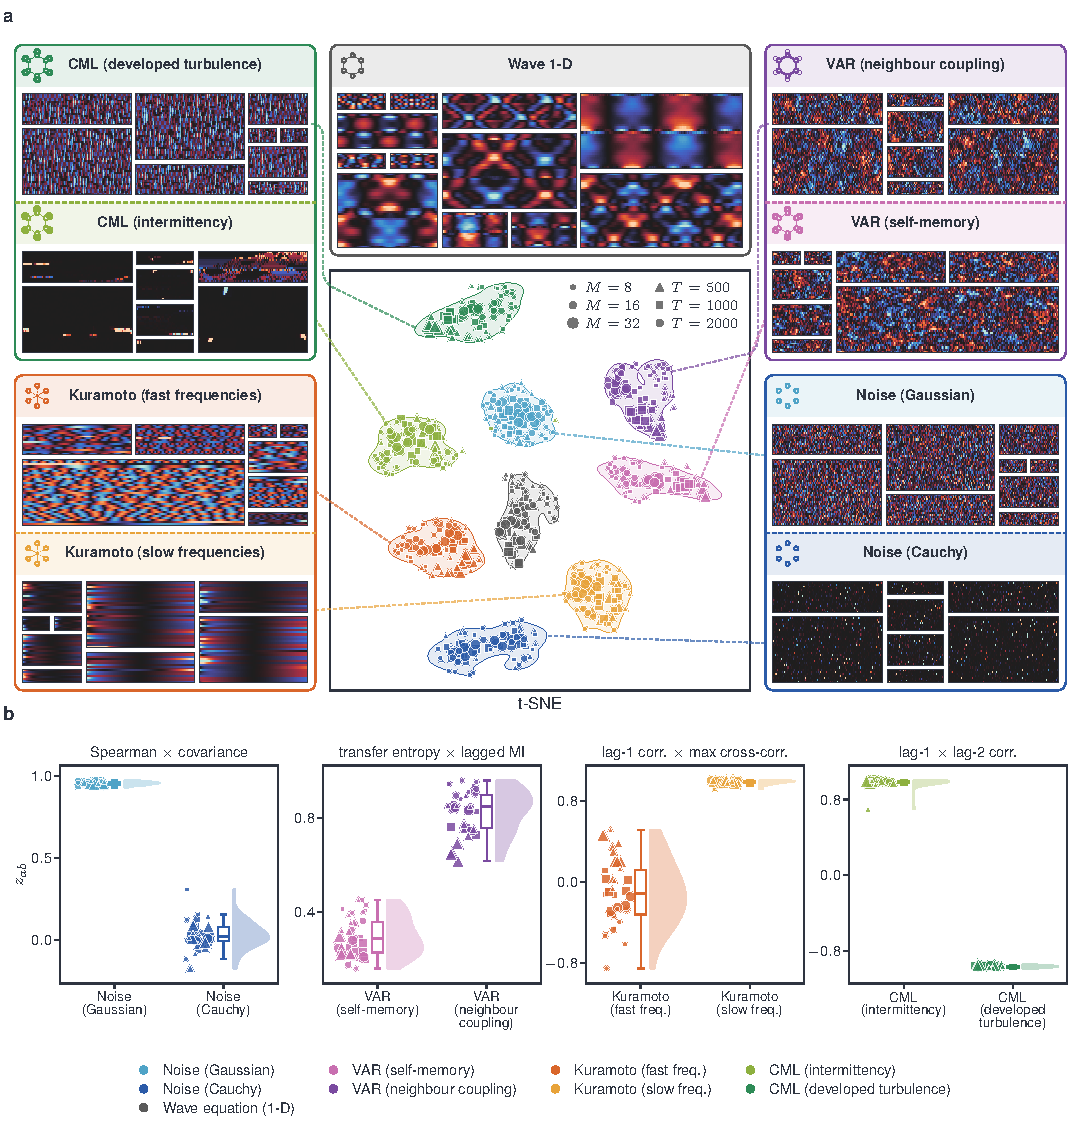
\includegraphics[width=.93\linewidth,height=.61\textheight,keepaspectratio]{proof-of-concept-legend}	% 2026-11-18 export (results/proof/figure-261029/proof-figure-legend.pdf)
% \centering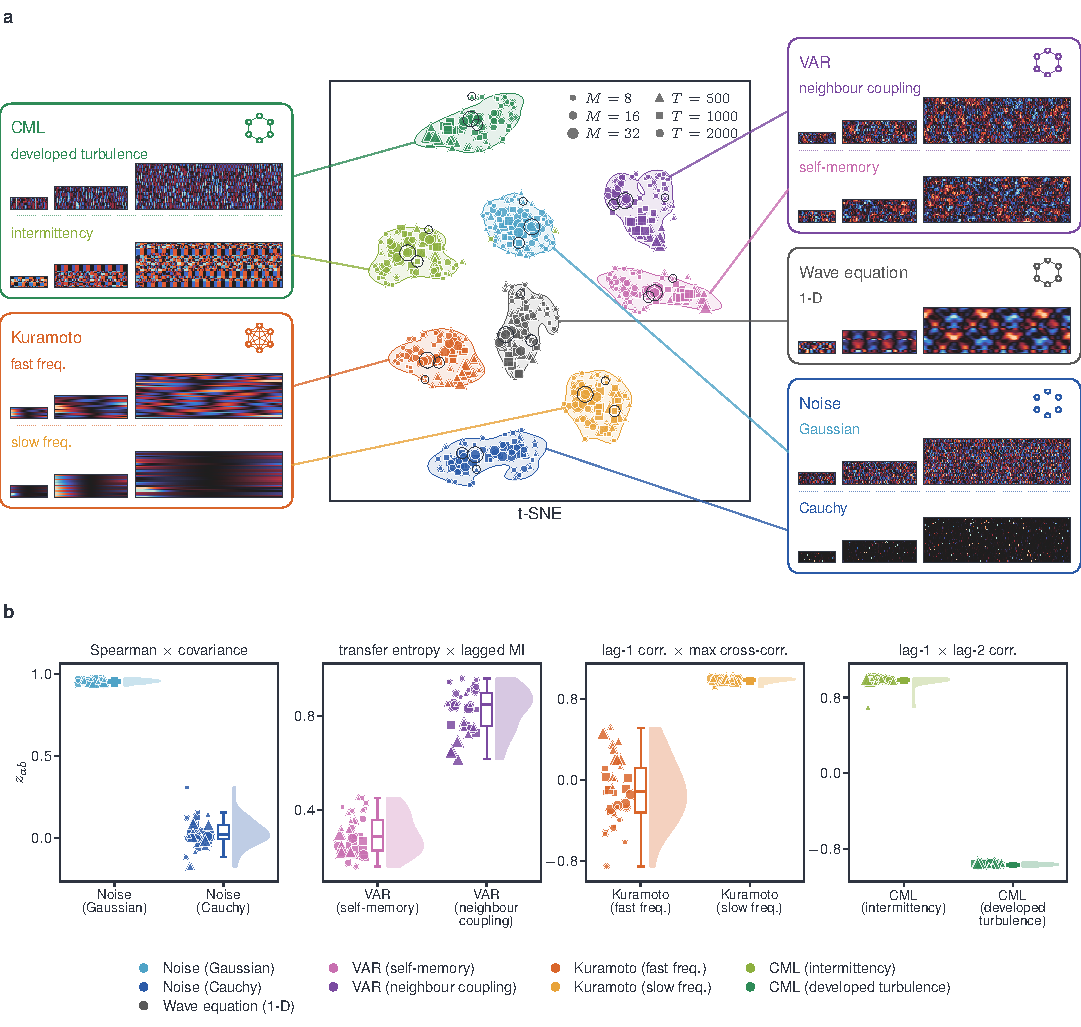
\includegraphics[width=.93\linewidth,height=.61\textheight,keepaspectratio]{proof-of-concept}	% previous version, outdated
\caption{\textbf{Different recording sizes occupy the same feature space.} The t-SNE display uses 23,176 retained coordinates. Colour denotes class, area channel count, and marker shape recording length. Example traces illustrate the generator families. Below, each coordinate compares a pair of variants across size cells, with selection and display using disjoint instances. Distances between islands have no calibrated physical scale.}
\label{fig:proof}
\end{figure}

\subsection{When a leading coordinate tracks a physical transition}

Two populations can become locked at a $2{:}1$ frequency ratio while their observed waveforms have almost zero linear correlation. This gives a demanding comparison because the physical target, the stability of the collective phase difference, is defined independently of the interaction statistics. We varied the coupling between two oscillator communities, added a third uncoupled community, and independently varied measurement noise between recordings. On 168 held-out recordings, the first principal component of centred profile correlations tracked the future locking index with absolute Spearman correlation $0.871$. The corresponding values for mean absolute Pearson correlation and the first component of per-statistic means were $0.032$ and $0.020$ (\cref{fig:order}). In clean recordings the leading component of the means also tracked locking. Varying measurement quality changed which source of variation dominated that representation.

The limits of this advantage are informative. In a finer Stuart--Landau sweep, the profile coordinate and the physical coherence changed most sharply in the same sampled interval, $0.720$--$0.725$. Mean absolute Pearson correlation tracked the order parameter at least as closely across the sweep ($0.915$ versus $0.886$). In a two-dimensional coupled map lattice the corresponding correlations were $0.966$ and $0.883$. In electronic oscillators the profile coordinate moved abruptly where late oscillators stopped slipping phase, yet mean edge strengths equalled or exceeded its rank association with the frequency range. These systems establish that collective order is accessible to a target-blind readout. The noisy locking experiment identifies a narrower advantage, when variation in signal quality dominates edge strengths but leaves enough of their relative organisation intact.

\begin{figure}[htbp]
\centering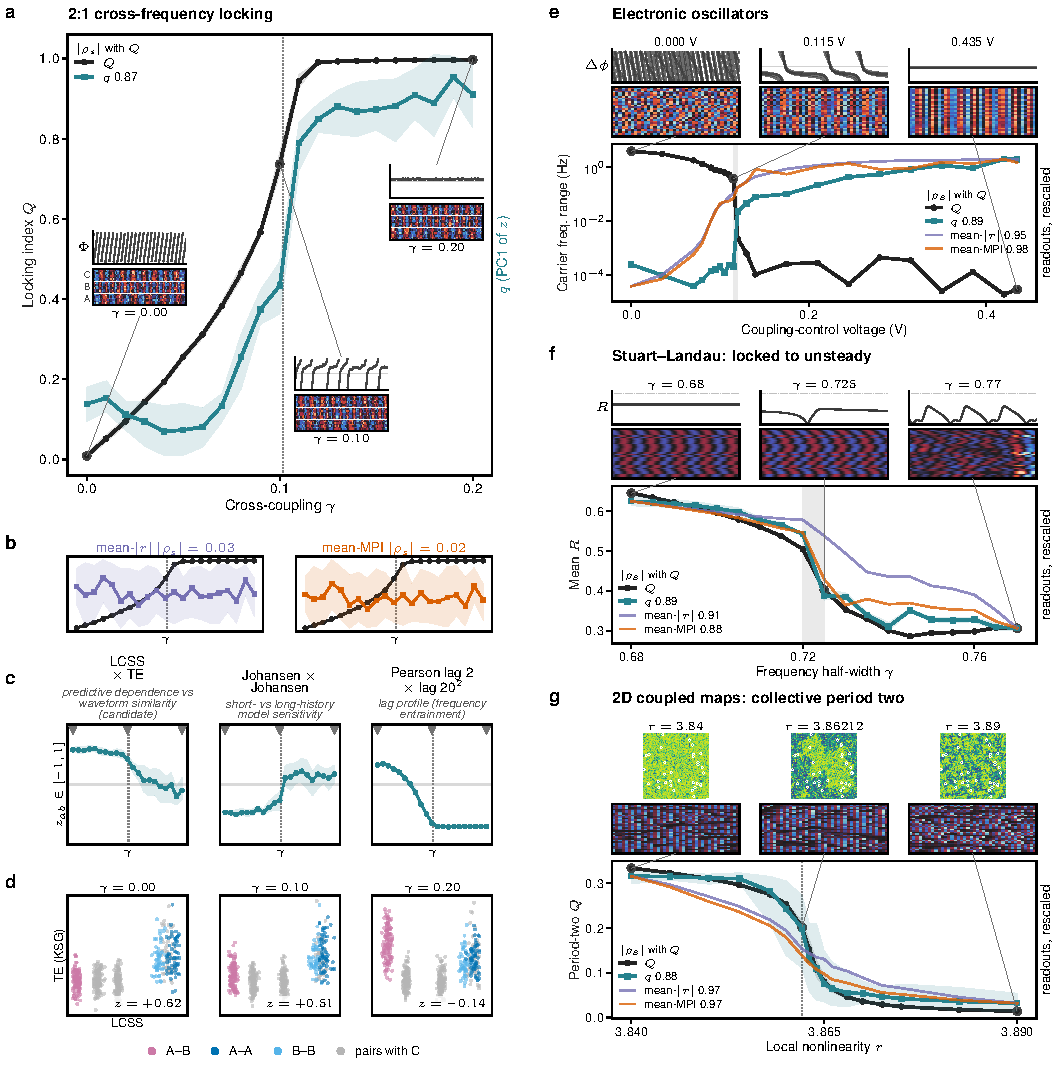
\includegraphics[width=\linewidth,height=.63\textheight,keepaspectratio]{order-parameter-inference}
\caption{\textbf{A target-blind coordinate compared with physical order.} In the locking experiment, $q$ is fitted without the locking index $Q$. The figure shows the transition, mean-strength comparators and the behaviour of selected edge profiles. Companion panels show hardware, a fine Stuart--Landau sweep and a two-dimensional coupled map lattice. Curve scales are chosen separately for display. Agreement with $Q$ is assessed on the original values.}
\label{fig:order}
\end{figure}

\subsection{Anaesthesia changes where Gaussian dependence predicts shared information}

In macaque electrocorticography, we asked whether the electrode pairs that share information are those expected from their linear correlation. We rank-transformed each channel to a standard normal marginal and estimated instantaneous MI twice on the same samples. The Gaussian estimate $G$ depends only on correlation. The nearest-neighbour estimate $K$ permits a more general joint distribution. A homogeneous Gaussian process can still yield imperfect agreement at finite sample size, particularly when its spectrum changes across states. We therefore measured $z(G,K)$ relative to a multichannel surrogate constructed separately for each window (\cref{fig:mi}).

Relative to eyes-closed wake, this surrogate-adjusted agreement fell in all 23 drug sessions. The session-mean changes were $-0.0159$ under ketamine (4 sessions), $-0.0155$ under ketamine--medetomidine (11), $-0.0062$ under medetomidine (4) and $-0.0117$ under propofol (4). Sleep gave a much smaller change, $-0.0010$ across seven sessions. For comparison, the between-session standard deviation of eyes-open minus eyes-closed residuals was $0.0020$. That scale describes the wake contrast. Biological replication is limited to four macaques, all with a negative pooled drug contrast (one-sided sign probability $1/16$, the minimum attainable with four animals; one-sided $t_3=-6.1$, $p=0.004$, on animal means). Only two received each single agent. Ketamine illustrates the contribution of the control especially clearly. Observed agreement fell by $0.0066$, although the matched-surrogate agreement \emph{rose} by $0.0093$.

\begin{figure}[htbp]
\centering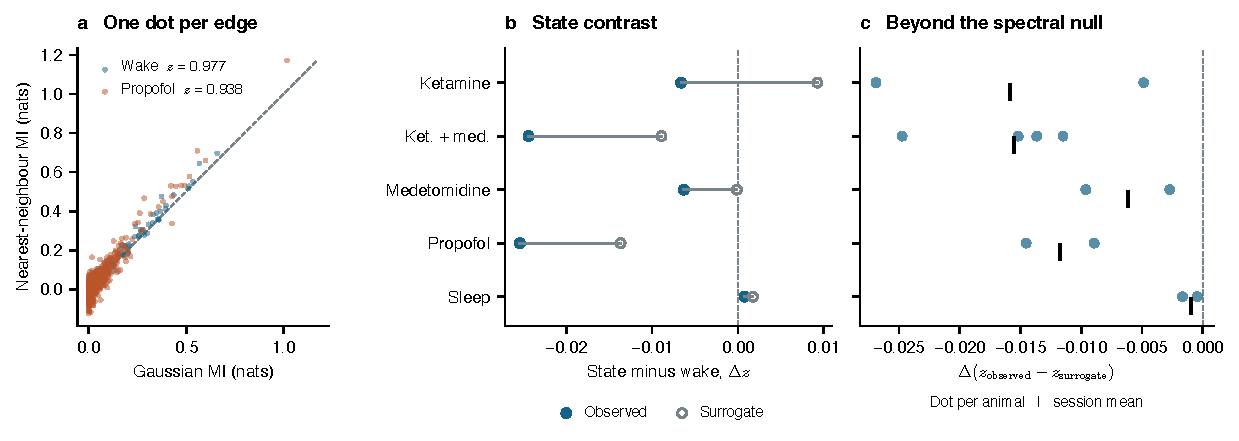
\includegraphics[width=\linewidth]{mi-character}
\caption{\textbf{Which edges share more information than Gaussian correlation predicts?} (a) Each point is one of 496 pairs among 32 channels, from a representative wake or drug window of the first propofol date. The diagonal marks equal MI estimates. (b) The state contrast in agreement is estimated in the recording and again in the matched surrogate. (c) Subtracting the latter gives the residual contrast. Each dot is an animal's mean over its sessions for that condition; the vertical tick is the mean over sessions. Sleep also uses eyes-closed wake as its reference.}
\label{fig:mi}
\end{figure}

The residual fall was robust to bipolar re-referencing under ketamine, the combination and propofol. Recovery values approached baseline. At all 126--127 retained channels, the same change coexisted with opposite movements in \emph{level}. Mean kNN MI in excess of the matched surrogate rose by $0.015$ nats under ketamine and fell by $0.013$ under propofol and $0.008$ under the combination. Removing on held-out windows the top $1\%$ of edges selected for their contribution to the change retained $127\%$ of the original fall. A small group of unusually influential edges is thus insufficient to explain the profile result. Nor did the fall depend on the nearest-neighbour setting: with ten neighbours, or with a Gaussian-kernel estimate in place of $K$, against the same surrogates, the animal means remained negative in all four macaques (pooled drug changes $-0.0126$ and $-0.0100$, against $-0.0133$ with four neighbours; one-sided $p=0.005$ and $0.014$).

Two further analyses bear on how the departure arises. Slow-wave activity is shared by anaesthesia and deep sleep. At equal delta-band fraction, a within-animal regression left the drug effects at $-2.2$ to $-3.5$ window-level eyes-open standard deviations under ketamine, ketamine--medetomidine and propofol ($-1.0$ under medetomidine), against $-0.2$ for sleep. Where drug and sleep windows overlapped in delta fraction, all eight drug sessions with windows in that range (ketamine and ketamine--medetomidine) gave $-3$ to $-4$ such units, against $-0.5$ for sleep. Slow-wave power therefore does not account for the change. Second, we repeated the surrogate separately within consecutive segments of each window. A segment surrogate admits linear-Gaussian dependence that differs between segments. With 5-s and 2-s segments the drug change was retained ($1.09$ and $0.96$ of its full-window value), which excludes drift across the window as its source. With 1-s segments $0.43$ remained, and with 0.5-s segments $0.29$, negative in all four animals at every length. In calibration, a static curved coupling retained $0.92$ at 1~s, whereas gain or coupling that changed over seconds retained $0.36$--$0.55$. Most of the departure therefore has the form of a mixture: dependence close to linear-Gaussian within a second, with a gain or coupling that differs between seconds. A smaller part persists below one second. The calibration did not separate these generators outright, so this describes the form of the departure, not its mechanism.

Mouse EEG provides a qualified test in another species \cite{claar2023}. Under sustained isoflurane, burst suppression can create the same signature through a shared amplitude envelope. During induction, a frozen follow-up selected windows with elevated delta power and with burst index above a prespecified awake threshold. All nine qualifying mice showed a decrease (mean $-0.0063$, mouse-bootstrap 95\% interval $[-0.0095,-0.0034]$). The result supports a departure during induction in continuous activity under that selection. Human propofol electrocorticography gave the same direction \cite{vanblooijs2023prios}. Seven patients with epilepsy were recorded awake on the ward and under propofol in theatre, in 2-s epochs between single-pulse stimuli. Between pulses the stimulated electrodes carry an identical signal, so after inspecting the data we left them out of each epoch. With every good channel and epoch the residual then fell in six of seven patients (mean $-0.0083$, 95\% interval $[-0.0163,-0.0002]$, one-sided $p=0.023$). In a sensitivity analysis declared before computing, it fell in all seven ($-0.0090$, $p=0.003$). The change was roughly 40--80\% of the macaque 2-s residual. Awake and propofol recordings came from different days and settings. A human sub-anaesthetic ketamine dataset gave a mean change near zero in seven patients (95\% interval $[-0.0053,0.0051]$) \cite{kauvar2025}. The evidence concerns particular states, recording modalities and doses.

\subsection{The same fall in directional share can conceal opposite changes in lead--lag structure}

The MI result suggests a more general question about paired statistics. Can a change in agreement be decomposed into the contributions of its two profiles? For temporal orientation there is an exact example. At a fixed delay, compare a matrix of lagged correlations with its transpose. A pair can share a large lagged correlation in both directions. Only the difference between those directions distinguishes which signal leads. The fraction of edge variation in that difference is exactly $(1-z)/2$. Time-reversal contrasts have previously distinguished brain states in these same macaques \cite{deco2022}. Here we separate the magnitude of the asymmetric component that recurs across windows from its share of all repeatable lagged structure.

At 20 ms, the mean repeatable asymmetric share fell under each drug, by 4.2--5.4 percentage points, and by 6.3 points in sleep (\cref{fig:lag}). Yet its absolute contribution rose under ketamine on all four dates and fell under propofol on all four dates and under the combination on all eleven. The ketamine and propofol dates included the same two animals. Under ketamine the symmetric component grew enough to dilute a growing asymmetric component. Under propofol the asymmetric component itself diminished. All-channel estimates and disjoint bipolar derivations preserved these three directions by date. When Fourier amplitudes were fixed to each date's wake spectrum, the absolute change remained positive on three of four ketamine dates and negative on every propofol and combination date. The group mean share then rose under ketamine. Thus the uniform fall in share depended on spectral weighting, whereas the drug contrast in repeatable asymmetric structure partly survived its removal.

This finding is exploratory and time-scale specific. At 40 ms the combination's mean absolute change became slightly positive on the primary montage. Eyes-open wake also changed the share, and recovery was incomplete for several agents. The ketamine increase was substantially larger in Chibi than in George. These properties make the measure a descriptor of temporal organisation at a stated lag. Inferring a propagation pathway would require additional spatial or interventional evidence.

We also applied the same 20-ms readout to awake and sustained isoflurane EEG in the independent mouse dataset, using the first eligible date per animal and all retained channels. With common-average reference the mean share fell from $5.48\%$ to $1.45\%$ (16/17 mice down), and mean repeatable asymmetric energy fell from $0.00341$ to $0.00097$ (16/17 down). With the as-recorded reference, the share fell in 17/17, but absolute energy fell in only 11/17. Thus the relative reorganisation extends to this burst-suppressed state. The absolute component is more reference-sensitive, and this comparison cannot establish an effect independent of bursting.

\begin{figure}[htbp]
\centering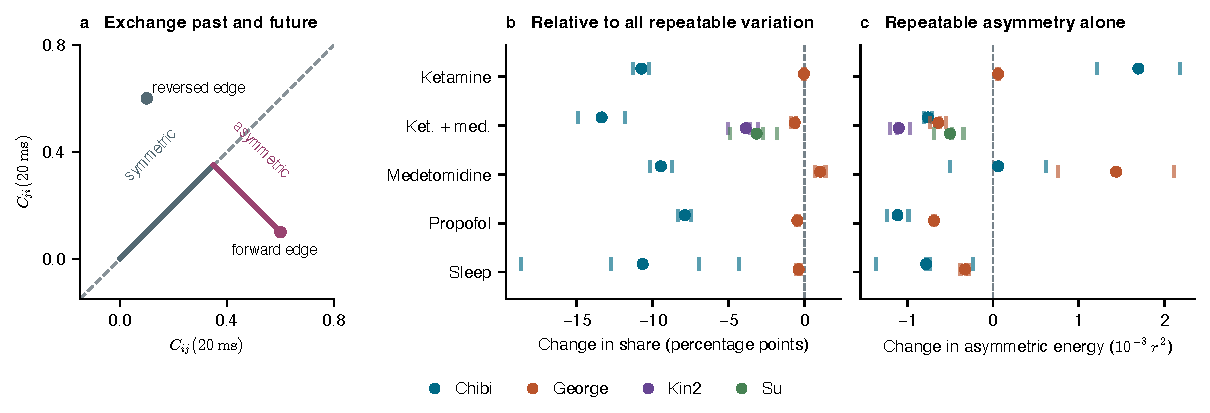
\includegraphics[width=\linewidth]{lag-reciprocity}
\caption{\textbf{A lag profile has two distinguishable components.} (a) For one illustrative pair, equal forward and reverse correlations lie on the diagonal. Its displacement perpendicular to that diagonal measures orientation asymmetry. (b) State minus eyes-closed wake for the share of lagged variation carried by recurring asymmetric edges. (c) The same contrast for absolute repeatable asymmetric energy. Short ticks are dates; dots are animal means. The same two animals contribute ketamine and propofol dates. Panels b and c use a 20-ms lag and common-average reference.}
\label{fig:lag}
\end{figure}


\section{Discussion}

The empirical MI contrast has a precise population reference. With continuous, normal-scored marginals, the excess of true MI over its Gaussian prediction at the same correlation equals the relative entropy from the covariance-matched bivariate Gaussian. Consequently, systematic departures are meaningful even in the absence of a proposed neuronal input--output law. Here the change concerns the organisation of those departures \emph{across} edges. An equal excess added to every edge leaves the correlation unchanged. The opposite changes in mean excess under ketamine and propofol make the distinction observable. We use \emph{nonlinear dependence} in the surrogate-data sense of a departure from the stationary linear-Gaussian expectation \cite{theiler1992testing,schreiber2000surrogate}. The window-matched contrast measures that departure under the stated constraints. In that tradition non-stationarity is the principal competing explanation \cite{schreiber2000surrogate}. Drift across the window is excluded here by the segment surrogates. Variation of gain or coupling within the window, which the segment analysis places on a timescale of about a second, is not an alternative to non-Gaussian dependence but one of its forms. The pooled samples of a window are then a mixture of Gaussians, which is not Gaussian; the gain example below is one case. Because almost any dynamics is close to linear-Gaussian over a short enough stretch, a segment surrogate locates the timescale of a departure rather than deciding whether it exists.

A direct measure addresses a different question. For an edge with positive true information $I$, $(I-G)/I$ is the fraction left unexplained by the Gaussian copula model. An invertible monotone transformation of a Gaussian pair can make a regression curve visibly nonlinear on the measurement scale and still give zero fraction after normal-scoring. For a complementary example, take independent standard Gaussian innovations $u,v$ and an independent, fluctuating positive gain $a$ with finite fourth moment. For $X=au$ and $Y=av$, $\operatorname{cov}(X,Y)=0$ yet $\operatorname{cov}(X^2,Y^2)=\operatorname{var}(a^2)>0$. The conditional mean of $Y$ given $X$ is identically zero. The dependence is in the magnitudes and survives invertible normal-scoring. Identifying curvature in a direct coupling law would require a model for the inputs, hidden state and measurement process, ideally tested by perturbing the putative source. A curved conditional regression fitted to observations alone would address a weaker question. A companion rank or monotonicity contrast on the measurement scale would expose sensitivity to a monotone observation map. In finite data a ratio needs a reliability criterion for $I$, a null estimate of the paired-estimator bias and a report of the fraction of edges for which a denominator is resolved. Truncating negative excess to zero before that assessment creates positive bias. A fixed threshold on noisy estimated MI can also select upward fluctuations in the ratio. Reporting excess in nats alongside any fraction preserves the distinction between a large relative change and substantial information.

Two consequences follow for interpreting a catalogue. First, a contrast has the clearest meaning when its two estimators differ in a property one can state and test. A lag tolerance, a conditioning set and a Gaussian approximation each permit a different counterfactual calculation on the same data. Second, a recording descriptor can usefully discard information. It can preserve a transition across a change of sensors or measurement quality, while losing a uniform strengthening of all edges or the anatomical identity of a critical pathway. When the scientific target is a particular connection, the edge profiles must be retained. For comparisons between recordings, their agreement instead answers a question about the system: which distinctions between forms of dependence organise its interactions?

\ifnature\section{Methods}
\label{sec:methods}

\paragraph{Edge profiles and their agreement.}
For a recording $X\in\mathbb{R}^{T\times M}$ and statistic $a$, let $v_a$ list its values $A^{(a)}_{ij}$ over all $i\ne j$ in a common order. Directed statistics retain both orientations. Duplicating the two orientations of an undirected pair leaves its correlation with another undirected profile unchanged. We define
\begin{equation}
z_{ab}=\frac{\langle v_a-\bar v_a,\ v_b-\bar v_b\rangle}{\|v_a-\bar v_a\|\,\|v_b-\bar v_b\|}.
\label{eq:z}
\end{equation}
The $K(K-1)/2$ coordinates of a $K$-statistic catalogue describe how estimates covary across edges. Pearson correlation preserves the sign and linearity of this correspondence. A common permutation of edge entries, including a channel relabelling, leaves the descriptor unchanged. A positive affine transformation of either profile also leaves it unchanged. Changing physical coupling can still reshape a profile and move $z$. A constant profile has undefined coordinates; nearly constant or unreliable profiles can give unstable ones. In the catalogue analysis we exclude invalid profiles for the recording and handle missing coordinates at the analysis stage. The edge count sets the dimension over which a correlation is measured and supplies no independent experimental replicates.

\paragraph{Controlled perturbations.}
The form experiment used 12 channels in blocks of four and $T=2000$. A common standardised AR(1) signal $u$ (coefficient $0.8$) was mixed with independent Gaussian channel noise, $w_i=(u+s_i\epsilon_i)/\sqrt{1+s_i^2}$, with the same four log-spaced noise levels $0.2$--$1.0$ per block. The first block observed $w_i$, the second either $w_i$ or $\sinh(2w_i)$, and the third either $w_i$ or $w_i^2$. After channel standardisation we computed empirical covariance (Pearson correlation), Spearman correlation and four-neighbour Kraskov MI \cite{kraskov2004}. The timing experiment used 15 channels in blocks of five and $T=1000$. Channels sampled a common smooth Ornstein--Uhlenbeck signal at $t-d_i(t)$ with additive noise. One block was aligned, one aligned or delayed by one to five samples, and one aligned or warped with $d_i(t)=A_i\sin(2\pi t/250)$ for $A_i=2,4,6,8,10$ samples. Every block used the same noise schedule ($0.1$--$0.4$). We compared normalised Euclidean distance, the minimum Euclidean distance over constant shifts (up to 250 samples), and normalised dynamic time warping. Each design used 20 independent seeds with paired draws across the four configurations.

\paragraph{Generative classification.}
The nine classes comprised independent Gaussian or Cauchy noise, two ring vector autoregressions, fast or slow repulsively coupled Kuramoto oscillators, two quadratic coupled map lattices, and a periodic one-dimensional wave equation. Each had ten realisations for every $(M,T)\in\{8,16,32\}\times\{500,1000,2000\}$. For the two autoregressions, self and per-neighbour coefficients were $(0.7,0.1)$ or $(0.2,0.35)$. The lattice map parameter and coupling were $(1.7522,0.00115)$ for intermittency and $(2,0.3)$ for developed turbulence. From the 283-statistic proof catalogue we reconstructed ordered edge-profile coordinates, kept those finite in at least 95\% of recordings, median-imputed missing values and removed coordinates of variance at most $10^{-8}$. The centred matrix yielded 50 principal components. The display used openTSNE 1.0.4, perplexity 30, five degrees of freedom and PCA initialisation (seed 260924). In a descriptive size-cell audit, the nearest-neighbour classifier excluded the target cell, but the unsupervised preprocessing and PCA saw all displayed recordings. For each within-family comparison we chose an interpretable coordinate with oriented training AUC at least $0.995$ in every size cell on instances 0--5. Instances 6--9 were used only for its displayed distributions and AUC.

\paragraph{Physical order.}
In the locking model, populations A and B of eight oscillators each interact through $2{:}1$ resonant coupling \cite{komarov2015}; a third eight-oscillator population has internal coupling only. We observed $\sin(\phi_i)$ for $1000$ samples and varied the A--B coupling over $0,0.01,\ldots,0.20$. The physical target was $Q=|\langle\exp[i(\Psi_B-2\Psi_A)]\rangle|$ from collective phases over a disjoint future interval. In the variable-noise arm, independent white measurement noise had one recording-specific standard deviation drawn uniformly from $0.3$--$0.9$ signal standard deviations. At each coupling eight independent seeds fitted the readouts and eight evaluated them. PCA used centred coordinates for $z$, and standardised edge means for the comparator from the same 289-statistic historical catalogue. The targets supplied an orientation for display. The Stuart--Landau comparison used 32 oscillators, coupling $0.8$, and a fine population-parameter sweep $0.680$--$0.770$ against mean phase coherence. The lattice comparison used 32 dispersed sites on a $256\times256$ lattice against a full-lattice period-two order parameter. Both used independently generated confirmation records. In the electronic oscillator data of Vera-\'{A}vila et al.\ \cite{vera2026}, carrier-frequency range indexed locking; the Erd\H{o}s--R\'enyi sweep supplied the fit and the small-world sweep a transfer comparison.

\paragraph{Gaussian reference and nonparametric MI.}
In each empirical MI window we normal-scored channel $i$ by $\Phi^{-1}[(\operatorname{rank}(x_i)-1/2)/T]$. For edge $e$ with normal-score correlation $r_e$, let $G_e=-\frac12\log(1-r_e^2)$ in nats. For continuous population variables with standard normal marginals and finite MI, $I_e-G_e=D_{\rm KL}(P_e\Vert\mathcal{N}(0,\Sigma_e))\geq0$, where $\Sigma_e$ is their nonsingular covariance matrix \cite{ince2017}. To see this, the Gaussian reference has the same marginal entropies and its log density is quadratic, with identical expectation under both distributions. The joint entropy difference is therefore precisely the KL divergence. The identity applies to population MI. Our flexible estimate $K_e$ used the same observations, four nearest neighbours and a pair-specific temporal exclusion radius from the autocorrelation functions (twice their inner product, integer-truncated and capped at $T/10$). Sampling error and estimator bias can give $K_e<G_e$.

\paragraph{Empirical windows, controls and unit of analysis.}
The NeuroTycho analysis used electrocorticography from four macaques \cite{yanagawa2013}. Signals were notch-filtered at mains frequency, band-limited to $0.5$--$40$ Hz, downsampled to 100 Hz and referenced to the mean of the retained channels. Nonoverlapping 10-s windows passed the atlas artefact screens. We compared eyes-closed wake with drug or sleep within each date, with eyes-open wake and recovery where available. The primary MI analysis used 32 dispersed contacts (496 undirected edges) and one multivariate iterative amplitude-adjusted Fourier-transform (IAAFT) surrogate per window. The final Fourier step retains each channel's spectrum and the between-channel phase differences at each frequency, hence the cross-spectra, while matching the normal-scored marginals approximately \cite{prichard1994generating,schreiber2000surrogate}. It randomises aspects of within-window timing that those constraints leave free. We averaged $R=z(G,K)_{\rm observed}-z(G,K)_{\rm surrogate}$ over windows within each date and state, then compared states within date and summarised dates within animal. An all-channel follow-up used three joint draws. Matched surrogates calibrate finite-window performance; one draw per window gives no tail probability for an individual edge or window.

In mouse isoflurane EEG (DANDI 000458), the induction follow-up required at least three stimulus-free windows with burst index (MAD/SD) at or above the awake fifth percentile and delta fraction at or above the awake 95th percentile for that animal. Nine of 17 mice qualified. The reference comprised its awake windows; three joint surrogates per window supplied the null and the interval resampled mice. The human comparison used pre-infusion and sub-anaesthetic infusion stereo-EEG from seven patients (DANDI 001347). Cross-species tests use participants as replicates and address the specified exposure and measurement conditions.

\paragraph{Reproducible lead--lag structure.}
At lag $\tau$ we computed the ordered matrix $C_{ij}=\operatorname{corr}(x_i(t),x_j(t+\tau))$. For each unordered edge set $S=(C_{ij}+C_{ji})/2$ and $A=(C_{ij}-C_{ji})/2$, orienting edges consistently across windows. Reversal of time exchanges $C$ and $C^\top$. With $S_c$ centred over unordered edges and $U=\|A\|^2$, $V=\|S_c\|^2$, the antisymmetric fraction $U/(U+V)$ equals $(1-z(C,C^\top))/2$ exactly on ordered edges. To measure the repeatable part, we replaced each mean square by the average dot product of the corresponding edge maps from distinct windows in the same date and state, divided by the number of edges. This removes the within-window noise square; correlated fluctuations across windows may still contribute. We report asymmetric energy and its fraction of repeatable total energy separately. The primary lag was 20 ms, with 10 and 40 ms as sensitivities. We used 32 dispersed channels and repeated the measurement on 32 disjoint index-neighbour bipolar differences. Post hoc checks used all retained channels and a Fourier reconstruction fixing each dispersed channel's amplitude spectrum to its date-specific root-mean-square awake spectrum while retaining its window-specific phases.

\paragraph{Data and implementations.}
Macaque data are from NeuroTycho. Mouse and human data are available from DANDI (000458 and 001347). The hardware sweeps are Zenodo records 17451096 and 17451530. The study repository contains the form and delay generators, the nine-class proof configuration, the locking and companion benchmark protocols, and the recording-level analysis scripts. The empirical MI calculation uses an explicit nearest-neighbour implementation with temporal exclusion. The lag calculation operates directly on the retained time series. Neither requires estimating the remainder of the SPI catalogue.
\backmatter\fi
\ifnature\else\bibliographystyle{unsrtnat}\fi
\bibliography{refs}
\end{document}
